%Input preamble
\input{preambleappendix}
%Other parameters
\newcommand{\noutcomes}{95}
\newcommand{\treatsubsabc}{$75\%$}
\newcommand{\treatsubscarec}{$74\%$}
\newcommand{\treatsubscaref}{$63\%$}

%Counts
%Males
\newcommand{\positivem}{$79\%$}
\newcommand{\positivesm}{$37\%$}

%Females
\newcommand{\positivef}{$73\%$}
\newcommand{\positivesf}{$35\%$}

%Counts, control substitution
%Males
\newcommand{\positivecsnm}{$58\%$}
\newcommand{\positivescsnm}{$25\%$}

\newcommand{\positivecsam}{$74\%$}
\newcommand{\positivescsam}{$38\%$}

%Females
%% no alternative
\newcommand{\positivecsnf}{$83\%$}
\newcommand{\positivescsnf}{$46\%$}

%% alternative
\newcommand{\positivecsaf}{$73\%$}
\newcommand{\positivescsaf}{$23\%$}

%Pooled

%Effects
%Males

%Females
\newcommand{\hsgradf}{$7$}
\newcommand{\yearsedf}{$1.2$}



%Pooled

%CBA
%IRR
%Males
\newcommand{\irrm}{$15\%$}
\newcommand{\irrsem}{$13\%$}

%Females
\newcommand{\irrf}{$10\%$}
\newcommand{\irrsef}{$12\%$}

%Pooled
\newcommand{\irrp}{$13\%$}
\newcommand{\irrsep}{$11\%$}

%BC
%Males
\newcommand{\bcm}{$7.88$}
\newcommand{\bcsem}{$8.06$}

%Females
\newcommand{\bcf}{$2.30$}
\newcommand{\bcsef}{$1.56$}

%Pooled
\newcommand{\bcp}{$4.35$}
\newcommand{\bcsep}{$2.57$}

%NPV streams
%Pooled
\newcommand{\parincomenpvp}{$\$115,026$}

\usepackage[stable]{footmisc}

\newcommand*\leftright[2]{%
  \leavevmode
  \rlap{#1}%
  \hspace{0.5\linewidth}%
  #2}

\newcommand{\orth}{\ensuremath{\perp\!\!\!\perp}}%
\newcommand{\indep}{\orth}%
\newcommand{\notorth}{\ensuremath{\perp\!\!\!\!\!\!\diagup\!\!\!\!\!\!\perp}}%
\newcommand{\notindep}{\notorth}


\begin{document}

\begin{titlepage}
\newgeometry{top=.8in, bottom=.8in, left=.8in, right=.8in}

\title{\Large \textbf{Gender Differences in the Benefits of a Prototypical Early Childhood Program: \\ Large Graphs of Gender Gaps}}

\author{
Jorge Luis Garc\'{i}a\\
Department of Economics\\
The University of Chicago \and
James J. Heckman \\
American Bar Foundation \\
Department of Economics\\
The University of Chicago \and
Anna L. Ziff \\
Center for the Economics of \\
Human Development \\
The University of Chicago}
\date{First Draft: January 5, 2016\\ This Draft: \today}

\maketitle
\restoregeometry
\end{titlepage}

\textbf{[JJH: These categories are never defined.][We now define them in Appendix C.]}


\textbf{[JJH: No difference [between IQ, achievement, parenting, social-emotional for controls]?][None of those are statistically different than 1/2.]}

\textbf{[JJH: Report p-values for each column.][We report the p-values testing if the control proportion is equal to the treatment proportion.]}

\textbf{[JJH: Report after treatment on control plot.][This is implemented. We replaced the previous figures (control and treatment separate) with Figure~\ref{fig:proportion}.]}

\textbf{[We no longer report the proportion value-added as the plots you suggested are much clearer.]}

\textbf{[We added a moderator of mother's locus of control (Figure~\ref{mlocus}). It shows that boys are hurt (relative to girls) when mothers have external loci of control. This is the case for all outcomes except health.}]

\begin{sidewaysfigure}[!htbp]
\centering
\caption{Proportion of Outcomes Males $>$ Females, by Outcome Category}
\label{fig:proportion}
	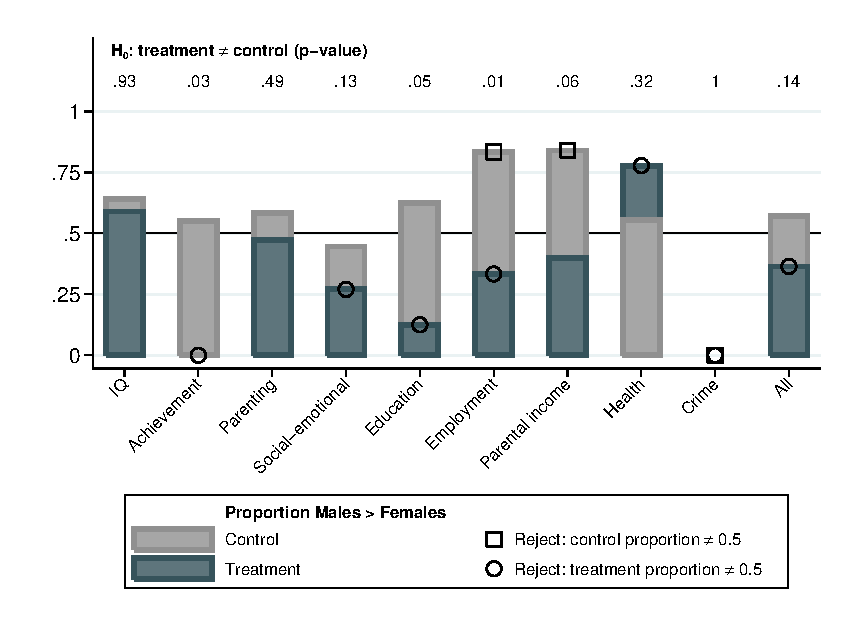
\includegraphics[width=\textwidth]{output/gendergaps-treat-vs-fullcontrol}
\footnotesize \justify
Note: These plots show the proportion of outcomes, by outcome category, for which the males' mean is larger than the females' mean. The standard errors and the $p$-values are computed using 100 bootstraps. The $p$-values are one-sided and test the null hypothesis that the proportion of outcomes is greater than $\frac{1}{2}$. All the variables are coded such that higher values correspond to socially desirable outcomes. The variables for each outcome category are listed in Appendix C.
\end{sidewaysfigure}

\begin{sidewaysfigure}[!htbp]
\centering
\caption{Proportion of Outcomes Males $>$ Females, by Outcome Category, Alternative Preschool}
\label{fig:proportion-alt}
	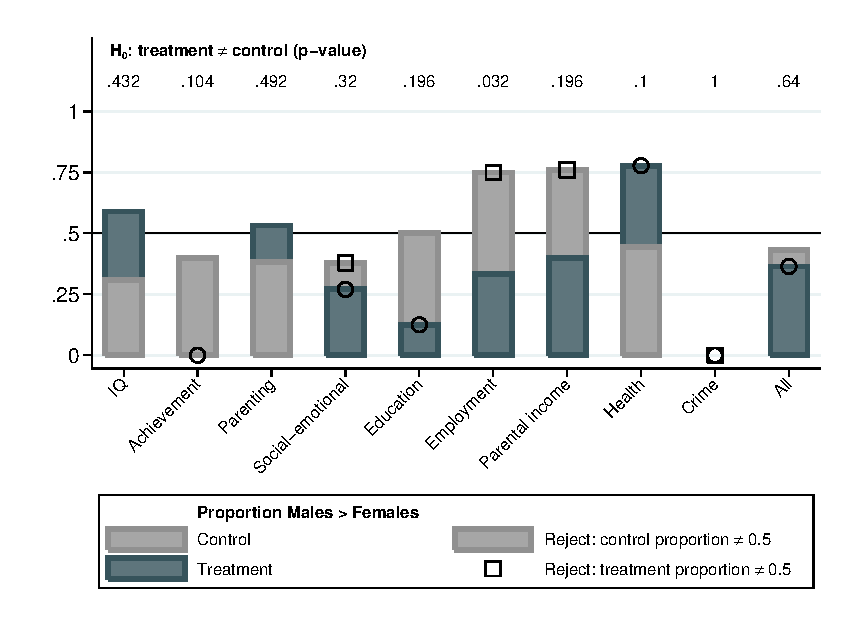
\includegraphics[width=\textwidth]{output/gendergaps-treat-vs-alt}
\footnotesize \justify
Note: These plots show the proportion of outcomes, by outcome category, for which the males' mean is larger than the females' mean. The standard errors and the $p$-values are computed using 100 bootstraps. The $p$-values are one-sided and test the null hypothesis that the proportion of outcomes is greater than $\frac{1}{2}$. All the variables are coded such that higher values correspond to socially desirable outcomes. The variables for each outcome category are listed in Appendix C.
\end{sidewaysfigure}

\begin{sidewaysfigure}[!htbp]
\centering
\caption{Proportion of Outcomes Males $>$ Females, by Outcome Category, Stay at Home}
\label{fig:proportion-home}
	\includegraphics[width=\textwidth]{output/gendergaps-treat-vs-home}
\footnotesize \justify
Note: These plots show the proportion of outcomes, by outcome category, for which the males' mean is larger than the females' mean. The standard errors and the $p$-values are computed using 100 bootstraps. The $p$-values are one-sided and test the null hypothesis that the proportion of outcomes is greater than $\frac{1}{2}$. All the variables are coded such that higher values correspond to socially desirable outcomes. The variables for each outcome category are listed in Appendix C.
\end{sidewaysfigure}

\begin{sidewaysfigure}[H]
\centering
\caption{Proportion of Outcomes Males $>$ Females, Control Group Divided by Home Status}\label{fig3}
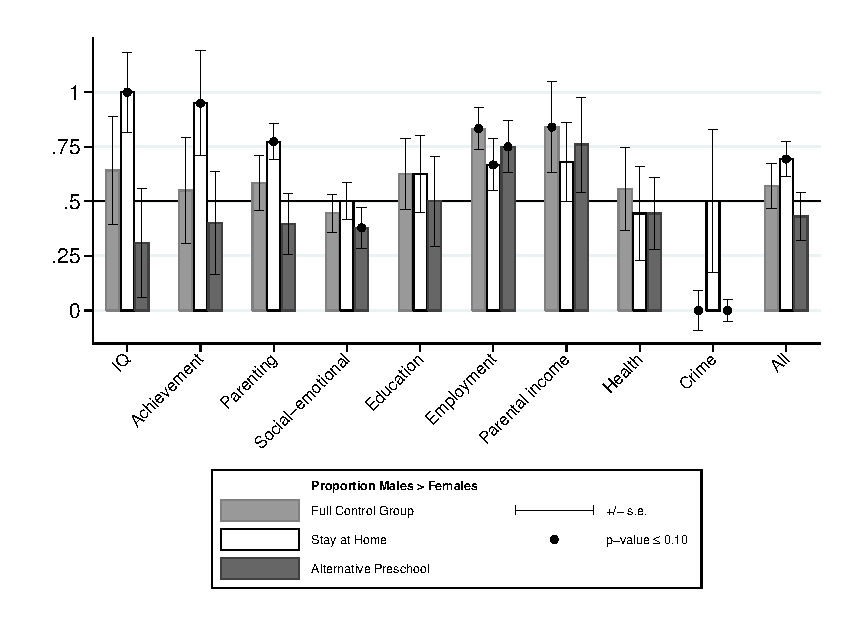
\includegraphics[width=\textwidth]{output/gendergaps-control-moderated-altpre}
\end{sidewaysfigure}

\begin{sidewaysfigure}[H]
\centering
\caption{Proportion of Outcomes Males $>$ Females, Control Group Divided by Father Present}
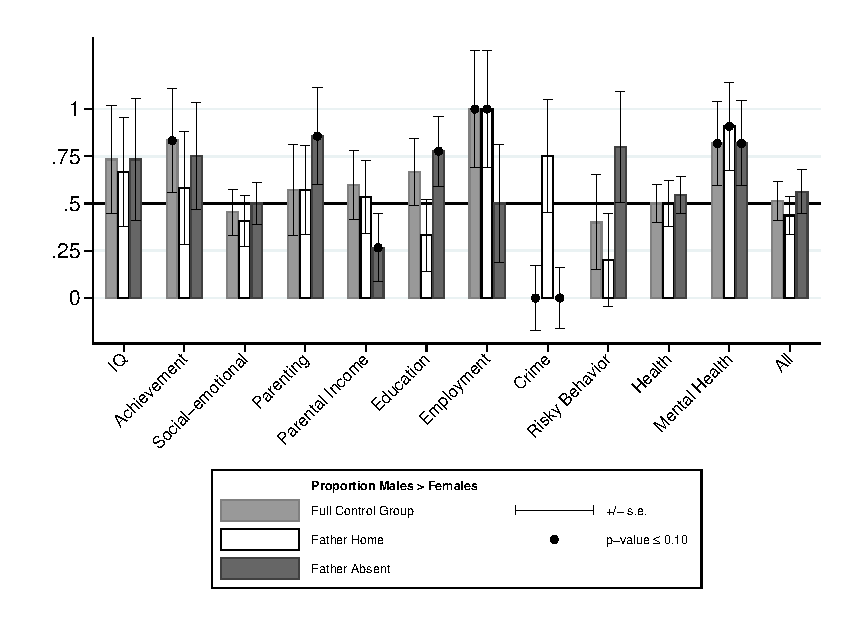
\includegraphics[width=\textwidth]{output/gendergaps-control-moderated-fhome}
\end{sidewaysfigure}

\begin{sidewaysfigure}[H]
\centering
\caption{Proportion of Outcomes Males $>$ Females, Treatment Group Divided by Father Present}
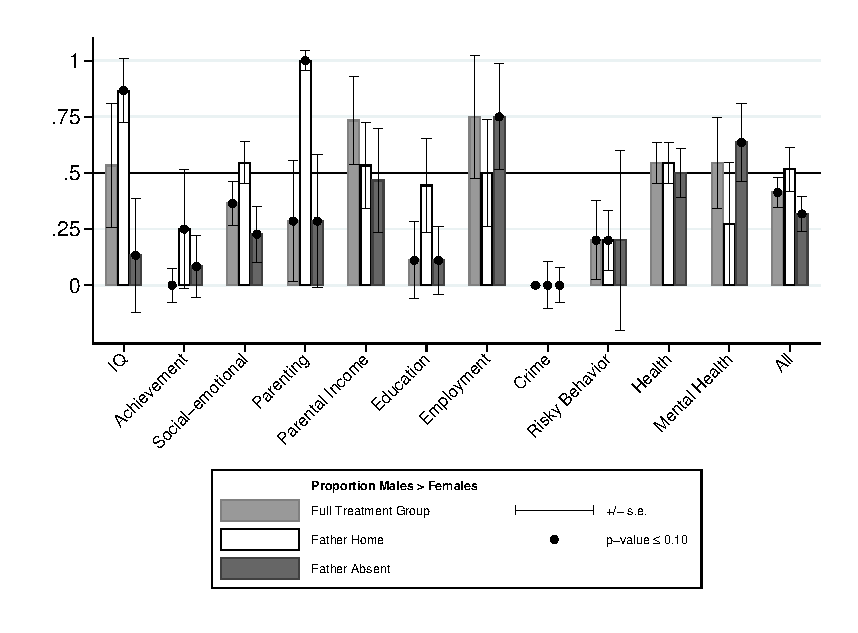
\includegraphics[width=\textwidth]{output/gendergaps-treatment-moderated-fhome}
\end{sidewaysfigure}

\begin{sidewaysfigure}[H]
\centering
\caption{Proportion of Outcomes Males $>$ Females, Control Group Divided by Mother's Locus of Control}
\label{mlocus}
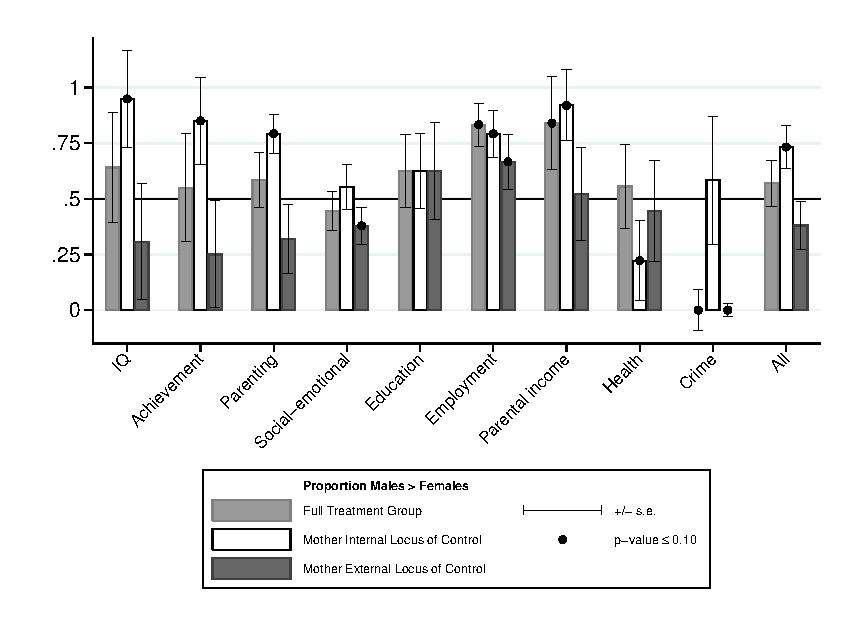
\includegraphics[width=\textwidth]{output/gendergaps-control-moderated-mlocus}
\end{sidewaysfigure}

\begin{sidewaysfigure}[H]
\centering
\caption{Proportion of Outcomes Males $>$ Females, Treatment Group Divided by Mother's Locus of Control}
\label{mlocus}
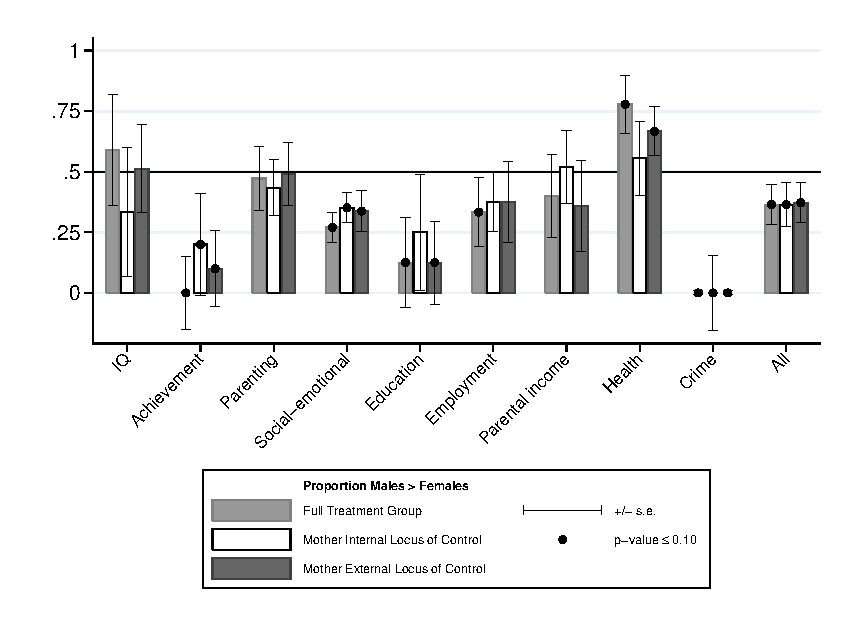
\includegraphics[width=\textwidth]{output/gendergaps-treatment-moderated-mlocus}
\end{sidewaysfigure}



\end{document}